\documentclass{beamer}

% NOTA:
%
% este ano não tenho tempo para melhorar isto. no próximo, isto tem que ficar
% mais parecido com a estrutura das aulas de L2R. Ou seja: fala-se no problema,
% faz-se um intervalo para dar o contexto (clustering) e depois fala-se nas
% aplicações (clustering de texto, clustering de resultados e descoberta de
% comunidades).

% melhorar a parte dos SOMs
% http://www.ai-junkie.com/ann/som/som5.html

%http://www.cse.psu.edu/~rcollins/CSE586Spring2010/papers/prmlMixturesEM.pdf
%
% em vez de MDS talvez wrod2vec?

\usepackage{pri}

\graphicspath{{./}{figures/}{figures/05-clustering-figs/}} 

\subtitle{Document Clustering and Dimensionality Reduction}

\begin{document}

\maketitle


% ------------------------------------------------------------

\begin{frame}
    \frametitle{Bibliography}
    \begin{block}{}
        \begin{itemize}
        \item \href{https://www.cs.uic.edu/~liub/WebMiningBook.html}{Bing Liu, Web Data Mining - Exploring Hyperlinks, Contents, and Usage Data.} Chapter 4.

        \item \href{http://nlp.stanford.edu/IR-book/}{Christopher D. Manning, Prabhakar Raghavan and Hinrich Schütze, Introduction to Information Retrieval,} Chapters 16 and 17.

        \item \href{http://www.mir2ed.org}{Ricardo Baeza-Yates and Berthier Ribeiro-Neto, Modern Information Retrieval,} Chapter 2.

        \item \href{http://www.mmds.org}{Jure Leskovec, Anand Rajaraman, and Jeff Ullman, Mining of Massive Datasets,} Chapters 7 and 11
        \end{itemize}
    \end{block}
\end{frame}

\section{Introduction}

\subsection{Motivation}

\begin{frame}
  \frametitle{Motivation}

  \begin{itemize}
  \item<+-> \textbf{Problem:} Query terms can be ambiguous
    \begin{itemize}
    \item E.g., query "star" retrieves documents about astronomy, animals, etc.
    \item<+->  Solution: \emph{clustering} document responses to queries along lines
      of different topics
    \end{itemize}
  \item<+-> \textbf{Problem:} Manual construction of topic hierarchies and
    taxonomies
    \begin{itemize}
    \item<+-> Solution: preliminary \emph{clustering} of large samples of web documents
    \end{itemize}
  \item<+-> \textbf{Problem:} Speeding up similarity search
    \begin{itemize}
    \item<+-> Solution: restrict the search for documents similar to a query to
      most representative \emph{cluster(s)}
    \end{itemize}
  \end{itemize}

\end{frame}

% ------------------------------------------------------------

\begin{frame}
  \frametitle{An Example}

  \centering
  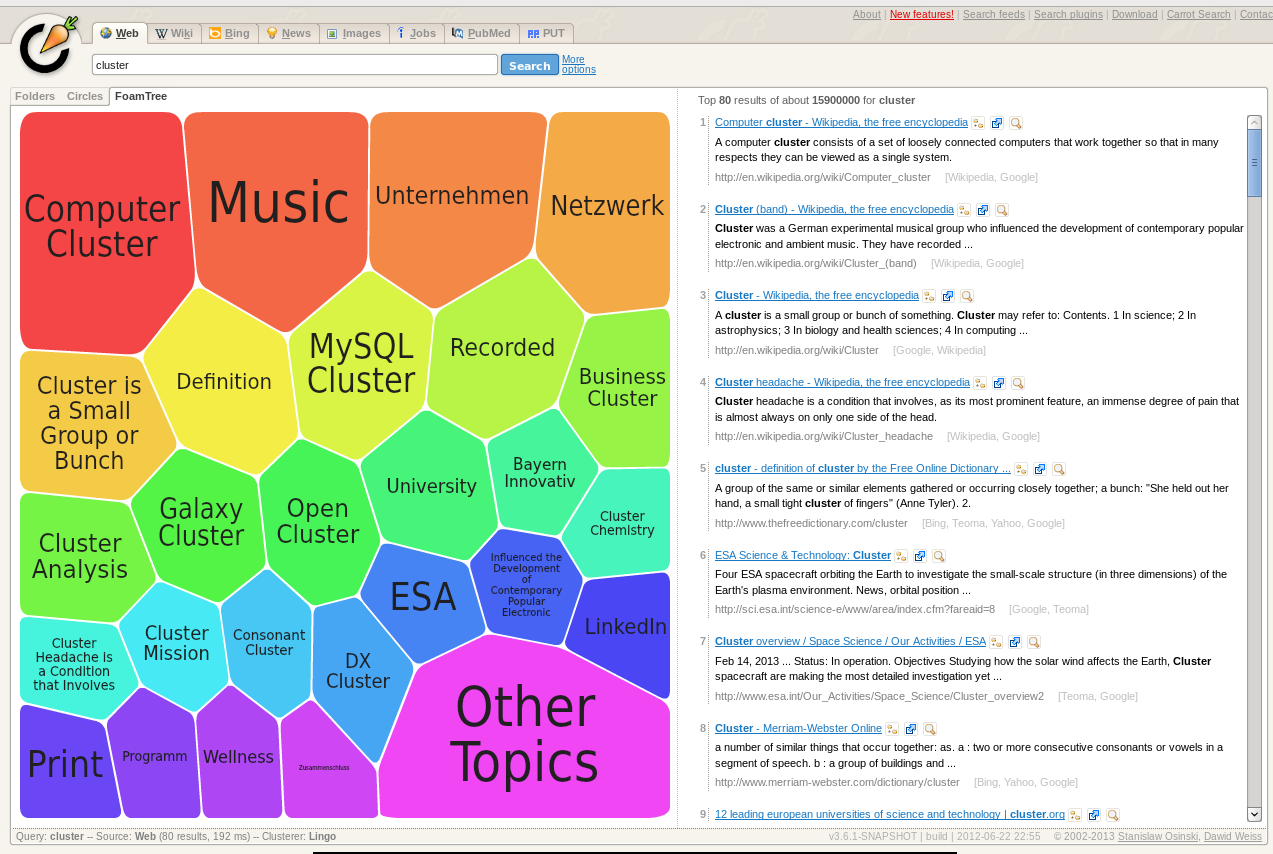
\includegraphics[width=\linewidth]{carrot}\\
  \footnotesize\url{http://search.carrot2.org}

\end{frame}

\begin{frame}
  \frametitle{Another Example}

  \centering
  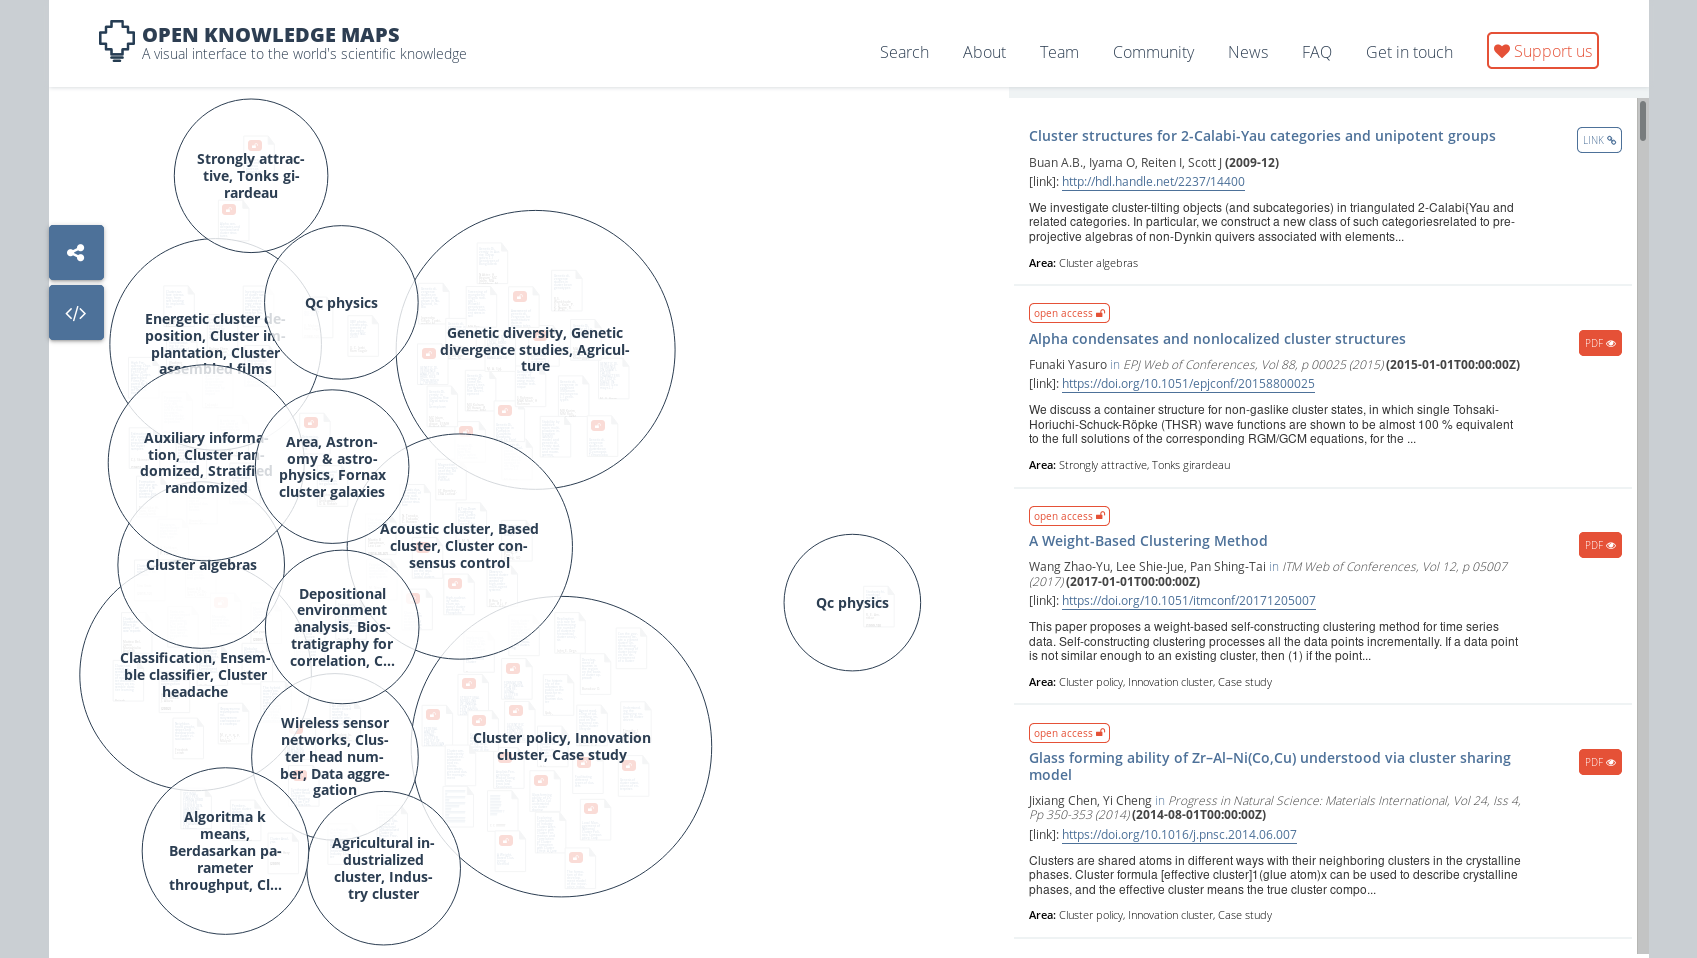
\includegraphics[width=\linewidth]{OKM}\\
  \footnotesize\url{https://openknowledgemaps.org/}

\end{frame}

% ------------------------------------------------------------

\begin{frame}
  \frametitle{Clustering}

  \textbf{Cluster Hypothesis:}
  \begin{itemize}
  \item Given a `suitable' clustering of a collection, if the user is
    interested in document $d$ (or term $t$), he is likely to be interested
    in other members of the cluster to which $d$ ($t$) belongs
  \end{itemize}

  \textbf{Clustering Task:}
  \begin{itemize}
  \item Use measures of similarity to \emph{cluster} a collection of
    documents/terms into groups, so that \emph{similarity within a cluster
      is larger than across clusters}
  \end{itemize}

\end{frame}

% ------------------------------------------------------------

\subsection{Basic Concepts}

\begin{frame}
  \frametitle{Clustering Concepts}

  \begin{itemize}
  \item Clustering paradigms:
    \begin{itemize}
    \item \emph{Bottom-up} agglomerative clustering
    \item \emph{Top-down} partitioning
    \end{itemize}
  \item Dimensionality reduction:
    \begin{itemize}
    \item Embedding of corpus in a low-dimensional space
    \item Many different approaches, based on heuristics, linear algebra, probabilistic models, ...
    \end{itemize}
  % \item Characterizing the entities to be clustered:
  %   \begin{itemize}
  %   \item Internally: Vector space model, probabilistic models
  %   \item Externally: Measure of similarity/dissimilarity between pairs
  %   \end{itemize}
  \end{itemize}

\end{frame}

% ------------------------------------------------------------

% \begin{frame}
%   \frametitle{Clustering Parameters}

%   General parameters:
%   \begin{itemize}
%   \item \emph{Similarity measure:} $\rho(d_1,d_2)$
%     \begin{itemize}
%     \item E.g., cosine similarity
%     \end{itemize}
%   \item \emph{Distance measure:} $\delta(d_1,d_2)$
%     \begin{itemize}
%     \item E.g., Euclidean distance
%     \end{itemize}
%   \item \emph{Number of clusters:} $k$
%   \end{itemize}

%   Problems:
%   \begin{itemize}
%   \item Large number of noisy dimensions
%   \item Notion of noise is dependent on the data and application 
%   \end{itemize}

% \end{frame}

% ------------------------------------------------------------

\begin{frame}
  \frametitle{Clustering Approaches}

  \begin{itemize}
  \item \emph{Partitioning Approaches}
    \begin{itemize}
    \item Bottom-up clustering
    \item Top-down clustering
    \end{itemize}
  \item \emph{Geometric Embedding Approaches}
    \begin{itemize}
    \item Self-organization map
%    \item Multidimensional scaling
    \item Latent semantic indexing
    \end{itemize}
  \item \emph{Generative models and probabilistic approaches}
    \begin{itemize}
    \item Single topic per document
    \item Documents correspond to mixtures of multiple topics
    \end{itemize}
  \end{itemize}

\end{frame}

% ------------------------------------------------------------

\section{Partitioning Approaches}

\begin{frame}
  \frametitle{Partitioning Approaches}

  \begin{itemize}
  \item Partition document collection into a set $G$ of $k$ clusters $[C_1, C_2, \dotsc,
    C_k]$
  \item Choices:
    \begin{itemize}
    \item Minimize intra-cluster distance: $\sum_i\sum_{d_1,d_2\in
        C_i}\delta(d_1,d_2)$
    \item Maximize intra-cluster semblance: $\sum_i\sum_{d_1,d_2\in
        C_i}\rho(d_1,d_2)$
    \end{itemize}
  \item If cluster representations $\vec{C_i}$ are available
    \begin{itemize}
    \item Minimize $\sum_i\sum_{d\in C_i}\delta(d,\vec{C_i})$
    \item Maximize $\sum_i\sum_{d\in C_i}\rho(d,\vec{C_i})$
    \end{itemize}
  \item Soft clustering
    \begin{itemize}
    \item $d$ assigned to $C_i$ with confidence $z_{d,i}$
    \item Find $z_{d,i}$ so as to minimize $\sum_i\sum_{d\in
        C_i}z_{d,i}\delta(d,\vec{C_i})$ or maximize $\sum_i\sum_{d\in
        C_i}z_{d,i}\rho(d,\vec{C_i})$
    \end{itemize}
  \item Two ways to get partitions: \emph{bottom-up clustering} and
    \emph{top-down clustering}
  \end{itemize}

\end{frame}

% ------------------------------------------------------------

\subsection{Bottom-Up Clustering}

\begin{frame}
  \frametitle{Hierarchical Agglomerative Clustering}

  \begin{itemize}
  \item Consider that $G$ represents a set of clusters
  \item Initially $G$ is a collection of \emph{singleton groups}, each with one
    document $d$
  \item Repeat
    \begin{itemize}
    \item Find $\Gamma,\Delta \in G$ with max similarity measure,
      $s(\Gamma \cup \Delta)$
    \item Merge group $\Gamma$ with group $\Delta$
    \end{itemize}
  \item Use above info to plot the hierarchical merging process
    (\emph{dendogram})
  \item To get desired number of clusters: cut across any level of the
    dendogram
  \end{itemize}

\end{frame}

% ------------------------------------------------------------

\begin{frame}
  \frametitle{Example Dendogram}

  \centering
  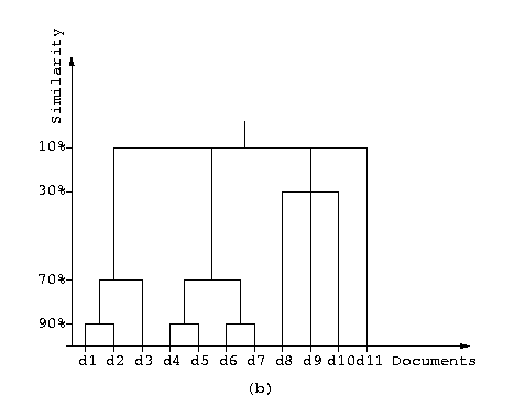
\includegraphics[width=.9\linewidth]{dendogram}  

  \raggedleft
  \tiny
  \href{http://www.bytemuse.com/post/crayon-hierarchical-clustering/}{(example)}
% http://harthur.github.io/clusterfck/demos/colors/

\end{frame}

% ------------------------------------------------------------

\begin{frame}
  \frametitle{Similarity Measures}

  \begin{itemize}
  \item Self-Similarity
    \begin{itemize}
    \item Consider that $\Phi$ represents a cluster
    \item Average pairwise similarity between documents in $\Phi$
      \begin{block}{}
        \begin{displaymath}
          s(\Phi) =
          \frac{1}{\binom{|\Phi|}{2}}\sum_{d_1,d_2\in\Phi}s(d_1,d_2)
        \end{displaymath}
      \end{block}
    \item $s(d_1,d_2)$ is the inter-document similarity measure (e.g., cosine
      of \textit{TF-IDF} vectors)
    \end{itemize}
  \item Other criteria:
    \begin{itemize}
    \item Maximum/minimum pairwise similarity between documents in the
      clusters
    \end{itemize}
  \item Complexity: $O(n^2\log{n})$ with $n^2$ space
  \end{itemize}

\end{frame}

% ------------------------------------------------------------

\subsection{Top-Down Clustering}

\begin{frame}
  \frametitle{Top-Down Clustering}

  \begin{itemize}
  \item Use an internal representation for documents as well as clusters (\emph{centroids})
  \item Partition documents into $k$ clusters
  \item 2 variants
    \begin{itemize}
    \item \emph{Hard:} 0/1 assignment of documents to clusters
    \item \emph{Soft:} documents belong to clusters with fractional scores
    \end{itemize}
  \item Termination
    \begin{itemize}
    \item When assignment of documents to clusters ceases to change much, or
    \item when cluster centroids move negligibly over successive
      iterations
    \end{itemize}
  \end{itemize}

\end{frame}

% ------------------------------------------------------------

\begin{frame}
  \frametitle{The $k$-Means Algorithm}

  \textbf{Hard $k$-Means}
  \begin{itemize}
  \item Choose $k$ arbitrary \emph{centroids}
  \item Assign each document to nearest centroid
  \item Recompute centroids
  \end{itemize}

  \begin{itemize}
  \item Contribution for updating cluster centroid
    \begin{block}{}
      \begin{displaymath}
        \Delta\mu_c = \sum_d\left\{
          \begin{array}{ll}
            \eta(d - \mu_c) & \text{if $\mu_c$ is closest to $d$} \\
            0 & \text{otherwise}
          \end{array}
        \right.
      \end{displaymath}
      \begin{displaymath}
        \mu_c \leftarrow \mu_c + \Delta\mu_c
      \end{displaymath}
    \end{block}
  \end{itemize}

\end{frame}

% ------------------------------------------------------------

\begin{frame}
  \frametitle{The $k$-Means Algorithm}

  \textbf{Soft $k$-Means}
  \begin{itemize}
  \item Don't break close ties between document assignments to clusters and
    don't make documents contribute to a single cluster which wins narrowly
    \begin{itemize}
    \item The contribution for updating cluster centroid $\mu_c$ from document
      $d$ is related to the current similarity between both
      \begin{block}{}
        \begin{displaymath}
          \Delta\mu_c = \eta\frac{1/|d-\mu_c|^2}{\sum_\gamma
            1/|d-\mu_\gamma|^2}(d - \mu_c)
        \end{displaymath}
      \end{block}
    \end{itemize}
  \end{itemize}

\end{frame}

% ------------------------------------------------------------

\begin{frame}
  \frametitle{An Example}
  
  \centering
  \href{http://www.cse.psu.edu/~rcollins/CSE586Spring2010/papers/prmlMixturesEM.pdf}{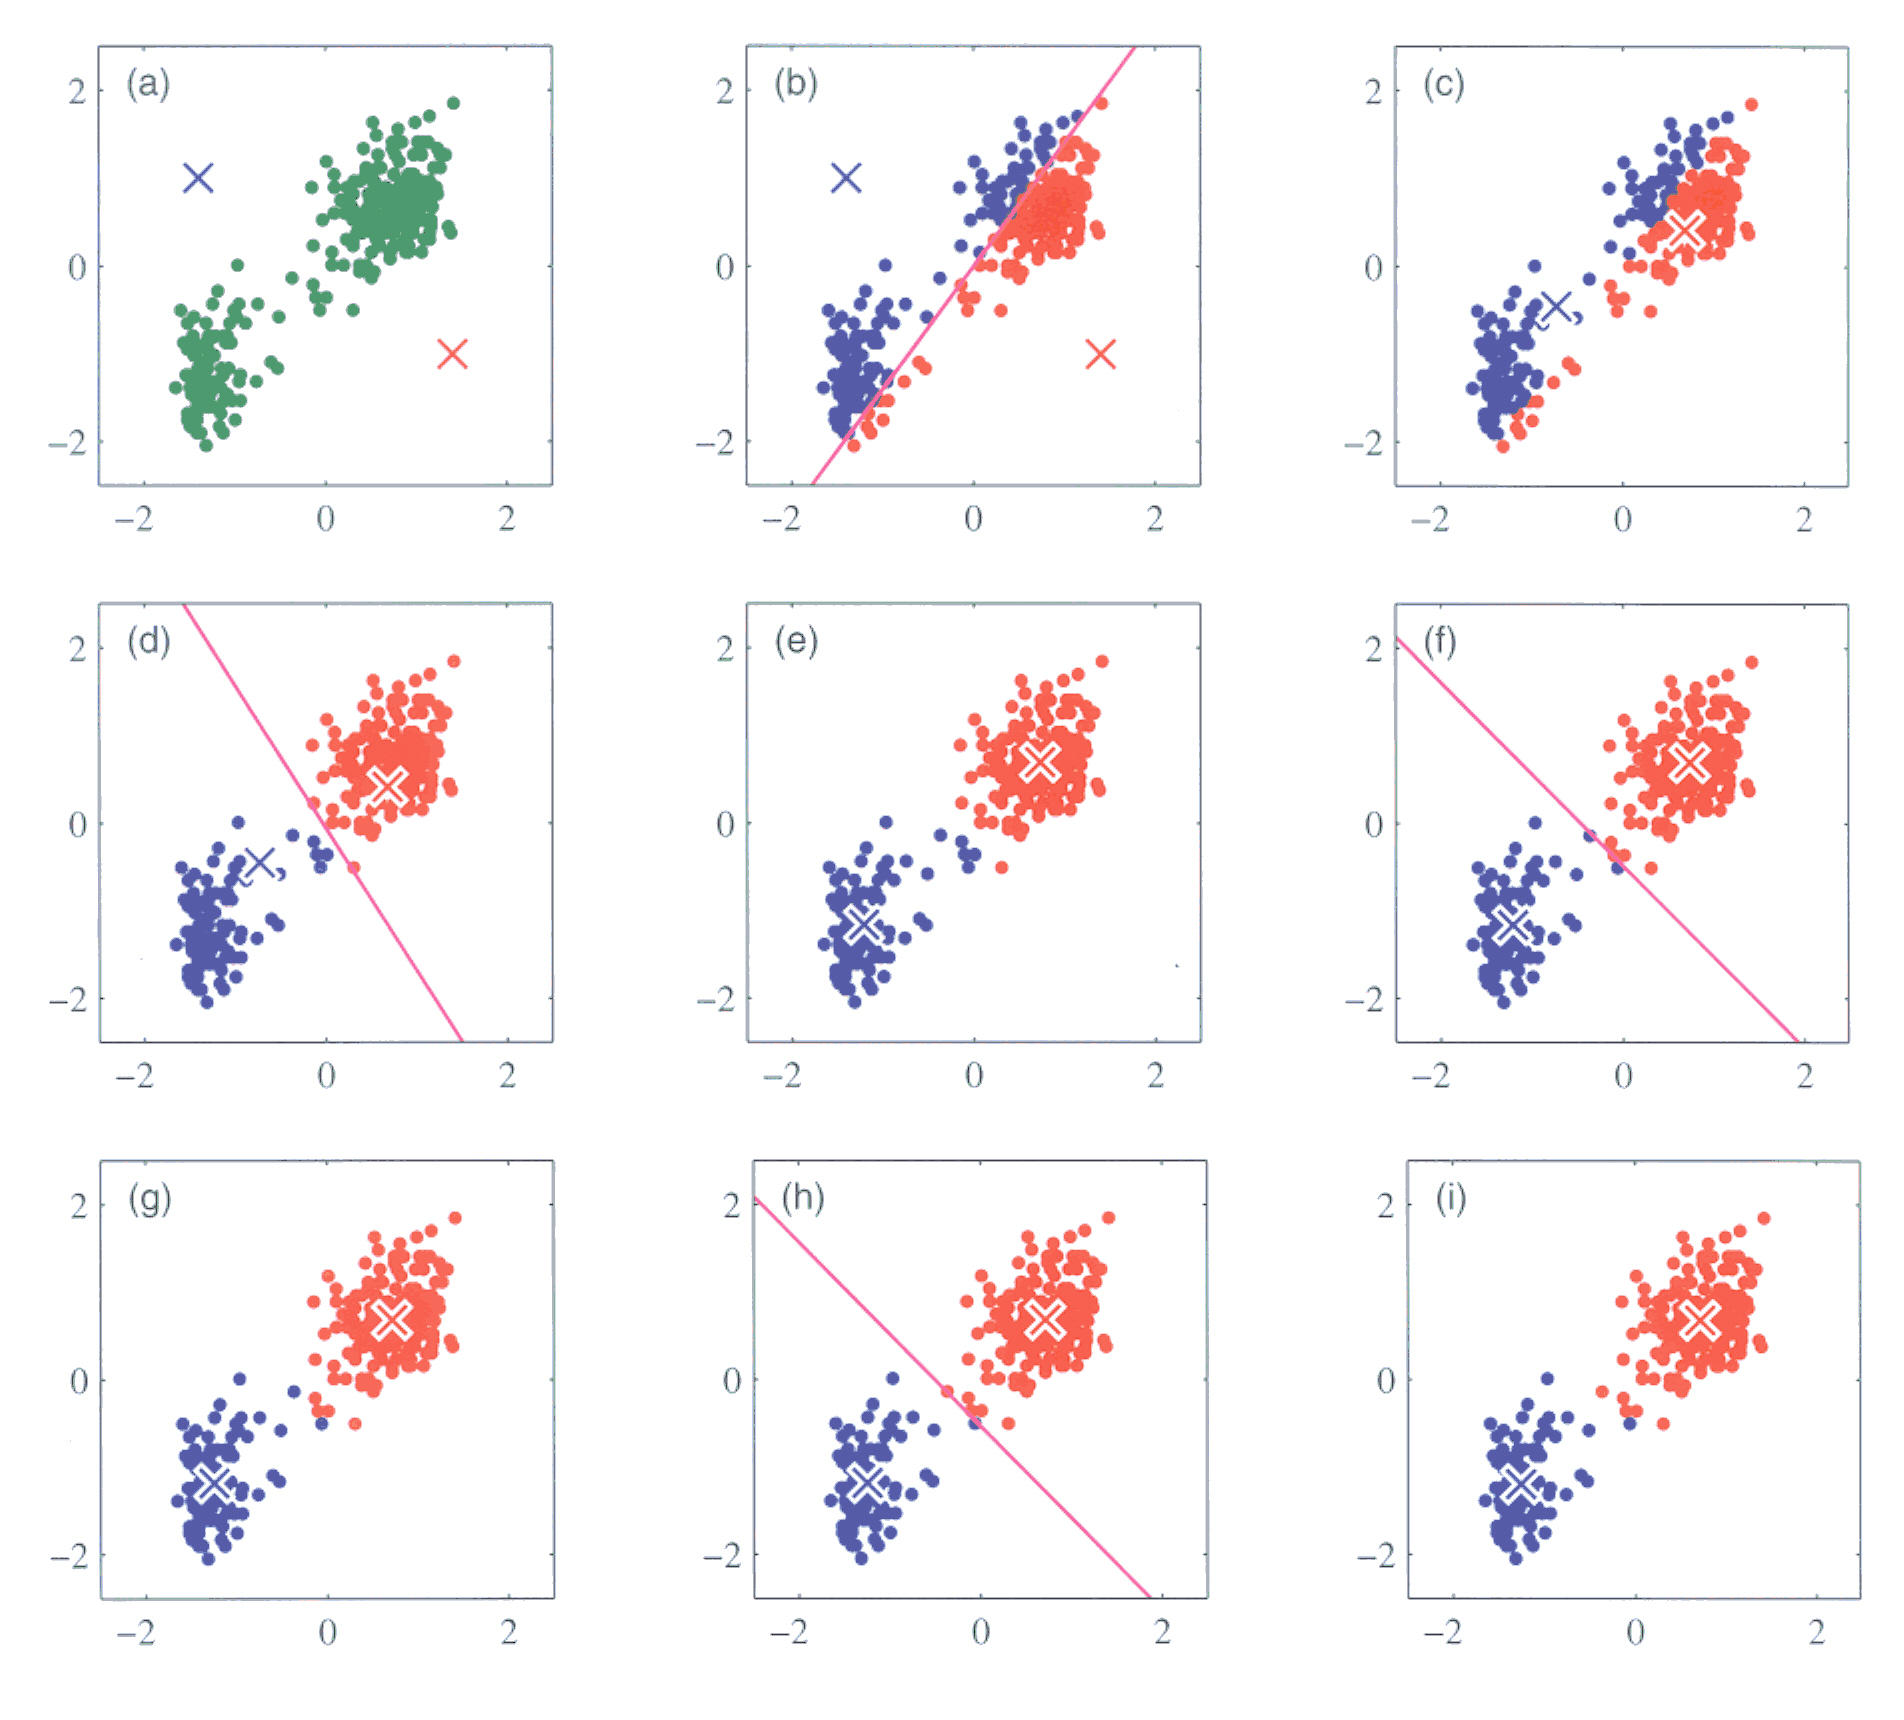
\includegraphics[height=.9\textheight]{k-means}}

  \raggedleft
  \tiny
  \href{http://mlehman.github.io/kmeans-javascript/}{(online demo)}
%\href{http://home.dei.polimi.it/matteucc/Clustering/tutorial_html/AppletKM.html}{(online demo)}
  %http://syskall.com/kmeans.js/
  %http://stanford.edu/class/ee103/visualizations/kmeans/kmeans.html
  % http://www.bytemuse.com/post/k-means-clustering-visualization/
\end{frame}

% ------------------------------------------------------------

% \begin{frame}
%   \frametitle{Complexity}

%   \begin{itemize}
%   \item Randomly sample $O(\sqrt{kn})$ documents
%   \item Run bottom-up group average clustering algorithm to reduce to $k$
%     groups or clusters: $O(kn\log n)$ time
%   \item Iterate $O(1)$ times
%   \item Move each document to nearest cluster
%   \item Recompute cluster centroids
%   \item Total time taken is $O(kn)$
%   \end{itemize}

% \end{frame}

% ------------------------------------------------------------

\section{Dimensionality Reduction}

\begin{frame}
  \frametitle{Dimensionality Reduction}

  \begin{itemize}
  \item \textbf{Goal:} Embedding of corpus in a low-dimensional space
  % \item Hierarchical Agglomerative Clustering (HAC)
  %   \begin{itemize}
  %   \item lends itself easily to visualization
  %   \end{itemize}
  \item \emph{Self-Organizing Map (SOM)}
    \begin{itemize}
    \item Technique related to $k$-means
    \end{itemize}
  \item \emph{Latent Semantic Indexing (LSI)}
      \begin{itemize}
      \item Linear transformations to reduce number of dimensions
      \end{itemize}
  \item Other techniques:
      \begin{itemize}
      \item Multidimensional scaling (MDS): Minimize the distortion of interpoint distances in the
          low-dimensional embedding as compared to the dissimilarity given in the
          input data
      \item NN-based word embeddings: Use neural networks to learn a mapping
          from the high dimensional vocabulary space to a lower dimension
          concept-based space
      \end{itemize}
  \end{itemize}

\end{frame}

% ------------------------------------------------------------

\subsection{Self-Organizing Maps}

\begin{frame}
  \frametitle{Self-Organizing Maps}

  \begin{itemize}
  \item Like soft $k$-means
    \begin{itemize}
    \item Determine association between clusters and documents
    \item Associate a representative vector with each cluster and iteratively
      refine
    \end{itemize}
  \item Unlike $k$-means
    \begin{itemize}
    \item Embed the clusters in a low-dimensional space right from the
      beginning
    \item A large number of clusters can be initialized even if eventually many
      are to remain devoid of documents
    \end{itemize}
  \item Each cluster can be a slot in a square/hexagonal grid.
    \begin{itemize}
    \item The grid structure defines the neighborhood $N(c)$ for each cluster
      $c$
    \end{itemize}
  \item Also involves a proximity function $h(\gamma,c)$ between clusters
  \end{itemize}

\end{frame}

% ------------------------------------------------------------

\begin{frame}
  \frametitle{Update Rule}

  \begin{itemize}
  \item Data item $d$ activates node (closest cluster) as well as the
    neighborhood nodes
    \begin{itemize}
    \item E.g., all nodes within $n$ hops
    \end{itemize}
  \item Update rule for node under the influence of $d$ is:
    \begin{block}{}
      \begin{displaymath}
        \mu_\gamma \leftarrow \mu_\gamma + \eta h(\gamma,c_d)(d - \mu_\gamma)
      \end{displaymath}
    \end{block}
  \end{itemize}
    
\end{frame}

% ------------------------------------------------------------

\begin{frame}
  \frametitle{A Self Organizing Map}

  \centering
  \href{https://codesachin.wordpress.com/2015/11/28/self-organizing-maps-with-googles-tensorflow/}{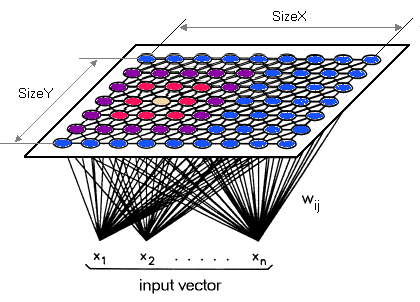
\includegraphics[width=\linewidth]{kohonen1}}

\end{frame}

% ------------------------------------------------------------

\begin{frame}
  \frametitle{Example}

  \centering
  \href{http://www.ai-junkie.com/ann/som/som5.html}{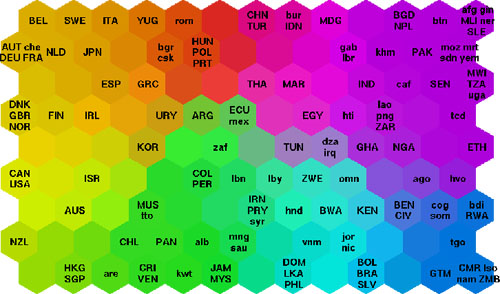
\includegraphics[width=\linewidth]{povertymap}}

\end{frame}

% ------------------------------------------------------------

\begin{frame}
  \frametitle{Example}

  \centering
  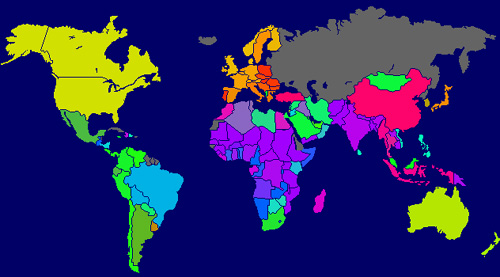
\includegraphics[width=\linewidth]{worldpovertymap}

  \raggedleft
  \tiny
  \href{https://irath96.github.io/som-demo/}{(online demo)}
\end{frame}

% ------------------------------------------------------------

% \subsection{Multidimensional Scaling}

% \begin{frame}
%   \frametitle{Multidimensional Scaling}

%   \begin{itemize}
%   \item \textbf{Goal:} \emph{Distance preserving} low dimensional embedding of
%     documents
%   \item Symmetric inter-document distances are given a priori or computed from
%     internal representation
%   \item Coarse-grained user feedback
%     \begin{itemize}
%     \item User provides similarity $d_{i,j}$ between documents $i$ and $j$
%     %\item With increasing feedback, prior distances are overridden
%     \end{itemize}
%   \item Objective : Minimize the stress of the embedding
%     \begin{block}{}
%       \begin{displaymath}
%         stress = \frac{\sum_{i,j}(\hat{d_{i,j}}-d_{i,j})^2}{\sum_{i,j}d_{i,j}^2}
%       \end{displaymath}
%     \end{block}
%   \end{itemize}

% \end{frame}

% % ------------------------------------------------------------

% \begin{frame}
%   \frametitle{Problems}

%   \begin{itemize}
%   \item Stress not easy to optimize
%   \item Iterative hill climbing
%     \begin{enumerate}
%     \item Points (documents) assigned ``random'' coordinates, e.g. by some external heuristic
%     \item Points moved by small distance in direction of locally decreasing stress
%     \end{enumerate}
%   \item For $n$ documents
%     \begin{itemize}
%     \item Each takes $O(n)$ time to be moved
%     \item Total $O(n^2)$ time per relaxation
%     \end{itemize}
%   \item Faster approach:
%     \href{http://www.cs.cmu.edu/~christos/software.html}{FastMap
%       [Christos Faloutsos and David Lin, 1995]}
%     % http://cs-people.bu.edu/evimaria/cs565/fastmap.pdf
%   \end{itemize}

% \end{frame}

% ------------------------------------------------------------

\subsection{Latent Semantic Indexing}

\begin{frame}
  \frametitle{Extended Similarity and LSI}

  \begin{itemize}
  \item In the vector space model different terms have different meanings
    \begin{itemize}
    \item car $\neq$ automobile
    \end{itemize}
  \item However, ``car'' and ``automobile'' are related
    \begin{itemize}
    \item They are likely to co-occur often
    \end{itemize}
  \item Documents having related words are related
    \begin{itemize}
    \item Useful for search and clustering
    \end{itemize}
  \item Two basic approaches:
    \begin{itemize}
    \item Hand-made thesaurus (e.g., \href{http://wordnetweb.princeton.edu/perl/webwn}{WordNet})
    \item Co-occurrence and associations
    \end{itemize}
  \end{itemize}

\end{frame}

% ------------------------------------------------------------

\begin{frame}
  \frametitle{Latent Semantic Indexing}

  \begin{itemize}
  \item Vector-space model
    \begin{itemize}
    \item Distinct orthogonal direction for each term
    \end{itemize}
  \item Not all terms are orthogonal
    \begin{itemize}
    \item E.g., ``car'' and ``automobile''
    \end{itemize}
  \item We need a matrix with a lower rank than the traditional document-term
    matrix, where similar terms are ``merged''
  \item This matrix can be found through \emph{Singular Value Decomposition}
  \end{itemize}

\end{frame}

% ------------------------------------------------------------

\begin{frame}
  \frametitle{Singular Value Decomposition}

  \centering
  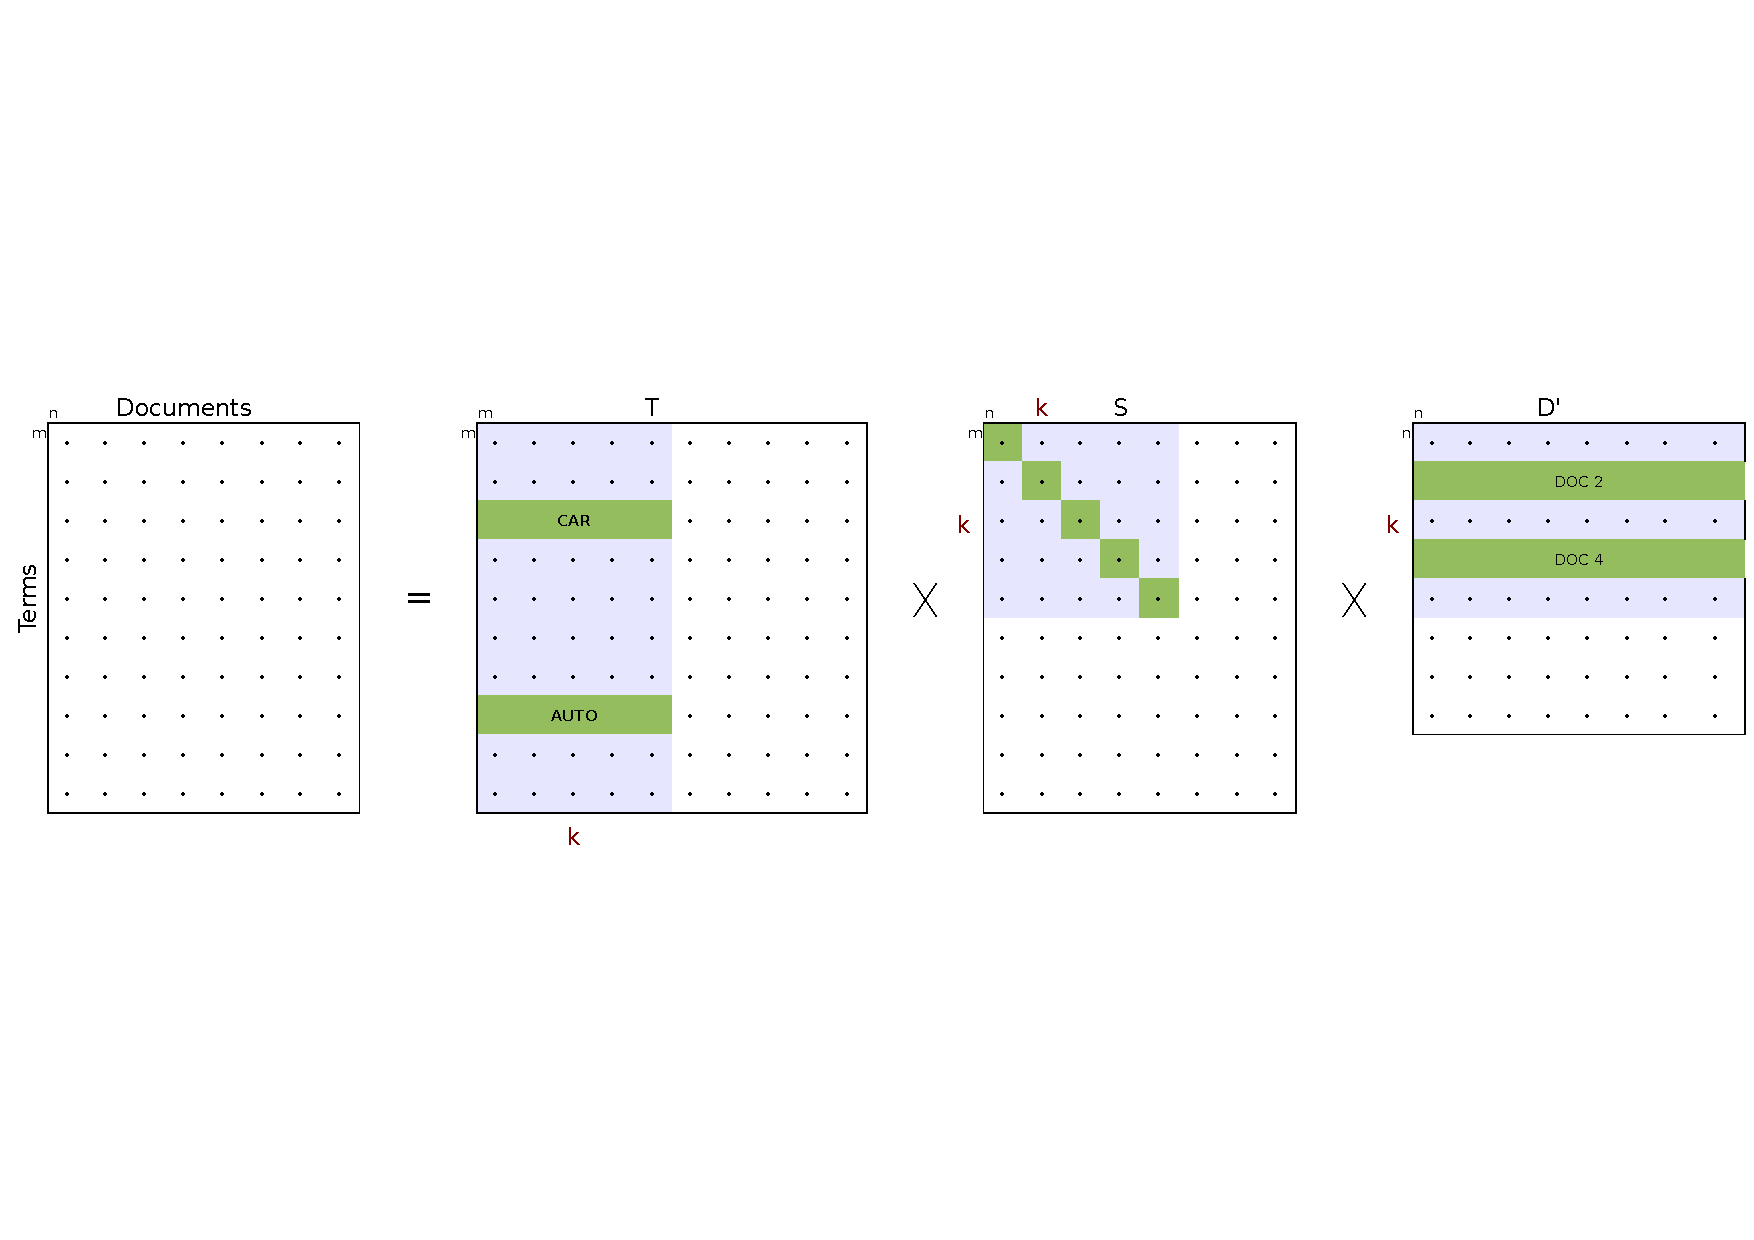
\includegraphics[width=\linewidth]{svd}

\end{frame}

% ------------------------------------------------------------

\begin{frame}
  \frametitle{Querying}

  \begin{itemize}
  \item $A = T \times S \times D^T \Leftrightarrow D = A^T \times T \times S^{-1}$
  \item A query $q$ is also projected to the new space
    \begin{block}{}
      \begin{displaymath}
        \hat{q} = q^T \times T \times S^{-1}
      \end{displaymath}
    \end{block}
  \item Cosine similarity can now be applied to the projections
  \item Results are often better than standard \textit{TF-IDF} retrieval/classification
    \begin{itemize}
    \item SVD filters out noise and ``discovers'' semantic associations between terms
    \item Representations in the projected vector space can be used for visualization
    \end{itemize}
  \end{itemize}

\end{frame}

% ------------------------------------------------------------

\begin{frame}
  \frametitle{Example}

  \centering
  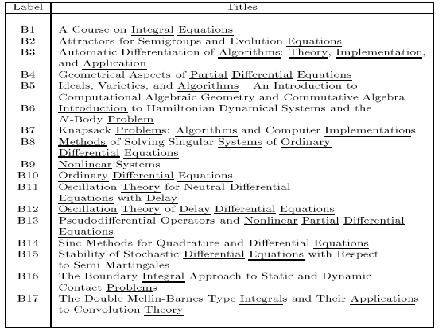
\includegraphics[width=\linewidth]{lsi1}

\end{frame}

% ------------------------------------------------------------

% TODO : change to something line https://liqiangguo.files.wordpress.com/2011/06/svd1.jpg
\begin{frame}
  \frametitle{Example}

  \centering
  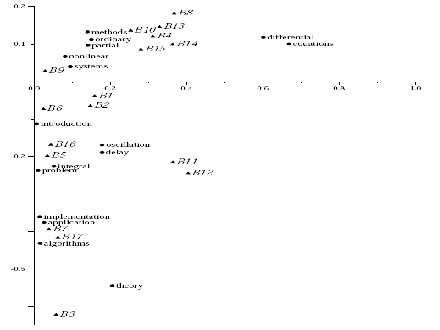
\includegraphics[width=\linewidth]{lsi2}

\end{frame}

% ------------------------------------------------------------

\begin{frame} 
  \frametitle{Problems}
  
  \begin{itemize}
  \item Exact solution is computationally expensive
    \begin{itemize}
    \item Can run in minutes to hours on a $10^3$ to $10^4$ collection
    \end{itemize}
  \item Approximation algorithms frequently used in practice
    \begin{itemize}
    \item Implementation in {\it scikit-learn} uses a fast randomized SVD solver [Halko , 2009]
    \end{itemize}  
  \item Most current implementations need to store the whole input matrix in memory
  \item Still not feasible for Web-sized collections
  \end{itemize}

\end{frame}

% ------------------------------------------------------------
% ------------------------------------------------------------

\finalframe{Questions?}

\end{document}
